
\documentclass[landscape,norsk,11pt]{seminar} 
 
\def\everyslide{\sf}
\usepackage{babel}
\usepackage{ucs}
\usepackage[utf8x]{inputenc}

\usepackage[T1]{fontenc}

\usepackage{hyperref}
\usepackage{graphics}

\slideframe{none}

\title{How to get the computer to manage natural language choices in a language learning process -- Linguistic and pedagogic problems}

\author{Lene Antonsen, Biret Ánne Bals Baal\\
Saara Huhmarniemi, Trond Trosterud \\
 \scalebox{0.10}[0.10]{
\includegraphics{img/LogoSamisk}}}
% \textit{http://giellatekno.uit.no/oahpa/}}
%  \scalebox{0.10}[0.10]{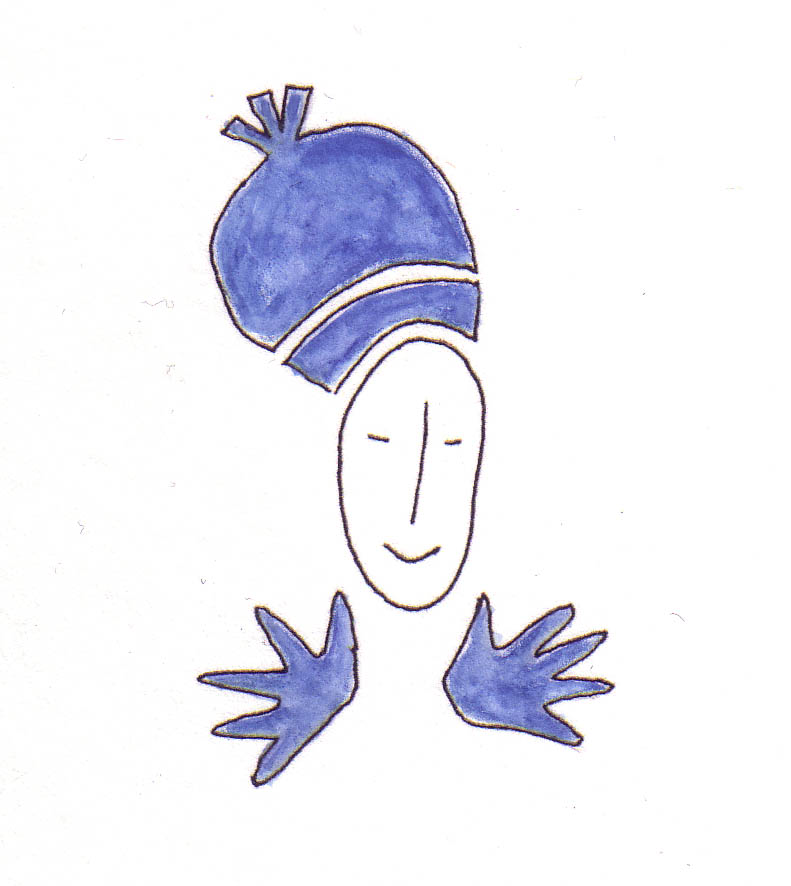
\includegraphics{img/vasta.png}} \\
\begin{document}
\begin{slide}

\maketitle


\newslide
\textit{http://giellatekno.uit.no/oahpa/}
\scalebox{0.30}[0.30]{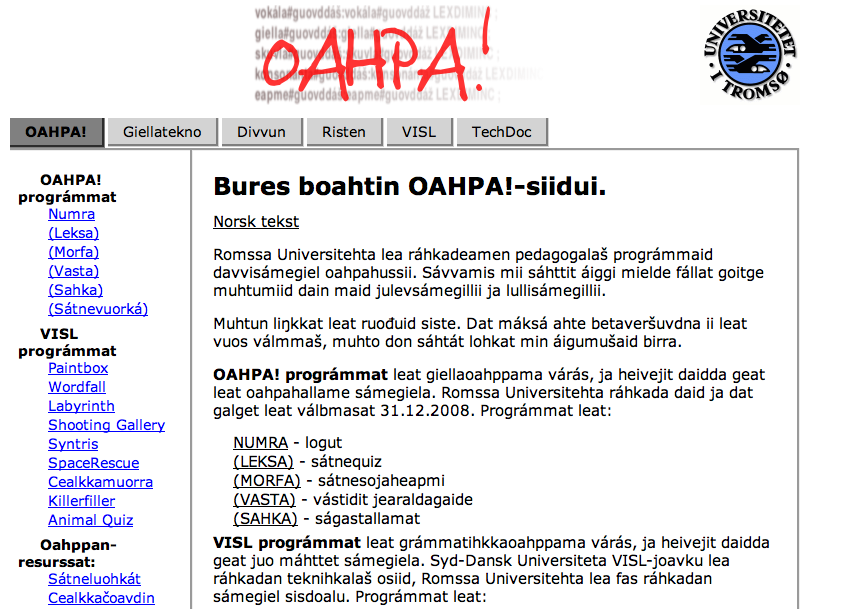
\includegraphics{img/gtoahpa.png}} 


\newslide
\textbf{VISL-programs - for grammar learning}\\
\newline
Word classes, syntax\\


\newslide
\textbf{OAHPA-programs - in order to learn Sámi}\\
\newline
\textbf{Leksa}: Sátnequiz - Sámi/Norwegian and Norwegian/Sámi\\
\textbf{Numra}: Exercise numerals\\
\textbf{Morfa}: Exercise word inflection, also contextual \\
\textbf{Vasta}: Exercise question anwering\\
\textbf{Sahka}: Participate in a dialogue on a given topic

\newslide
\textit{http://victorio.uit.no/oahpa/morfa/}
\scalebox{0.35}[0.35]{
\includegraphics{img/oahpa.png}} 

\newslide
\textbf{Vasta}
\scalebox{0.90}[0.90]{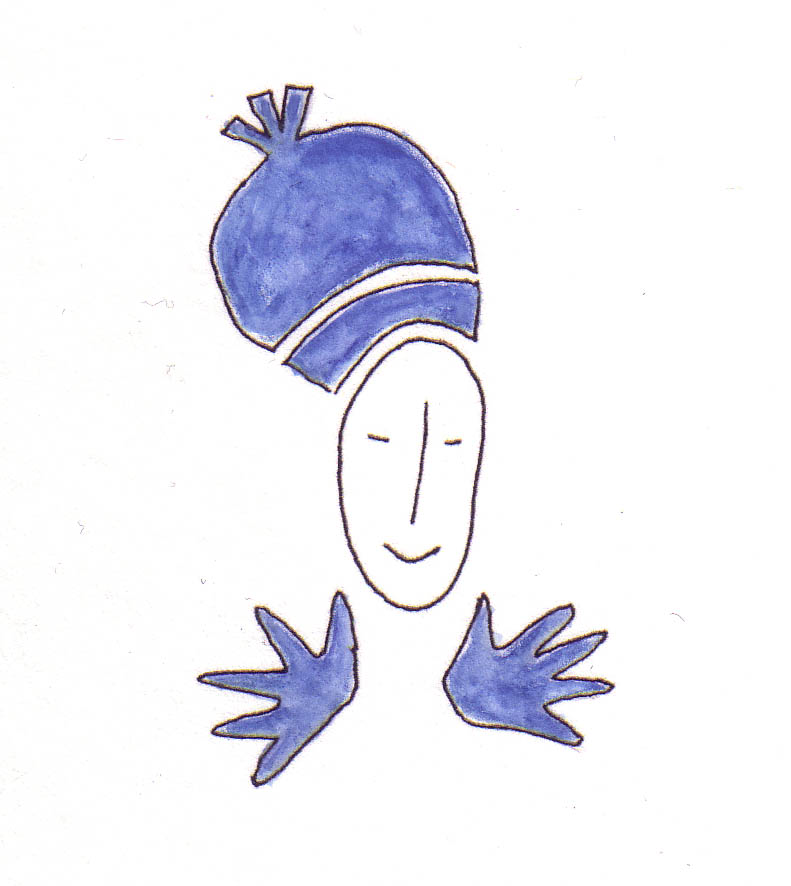
\includegraphics{img/vasta.png}} \\

%\newslide
%\textbf{Generating questions}
%\scalebox{.35}[.35]{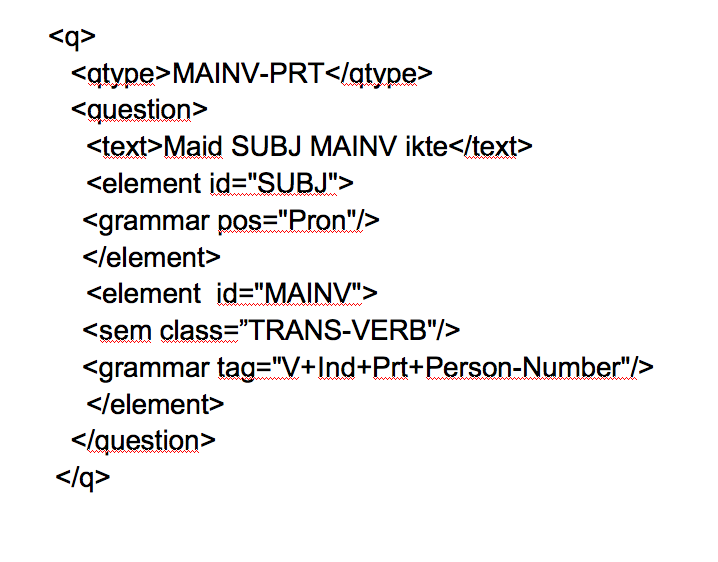
\includegraphics{img/xml_question.png}}

\newslide
\textbf{Pedagogical programs usually do not contain language technology, but rather} 
\begin{itemize}
\item multiple choice 
\item string -- e.g. \textit{viesus} = 6 marks 
\end{itemize}

\textbf{Language technology:} \textit{viesus} = viessu N Sg Loc 


\newslide
\textbf{Vision:}\\
The program should supervise the student in the same way as a teacher does.
\newslide
\textbf{E.g.: "Maid don lohket ikte?"} \\
Acceptable answers:
\begin{itemize}
\item Mun han lohken ollu áviissaid. 
\item Ikte mun gal lohken buori girjji. 
\item In lohkan maidege. 
\item Ikte in lohkan.
\end{itemize}

\newslide
\textbf{Maid don lohket ikte?}\\
The Vasta-program gives feedback if the answer is not acceptable:
\begin{itemize}
\item Mun lohket ollu \'aviissaid. \\ --> Husk kongruens mellom subjekt og verbal.
\item Mun lohken ollu \'aviissat. \\ --> Objektet skal være i akkusativ.
\item Don lohket ollu \'aviissaid. \\ --> Er du sikker på at du svarer i riktig person?
\end{itemize}

\newslide
\scalebox{0.13}[0.13]{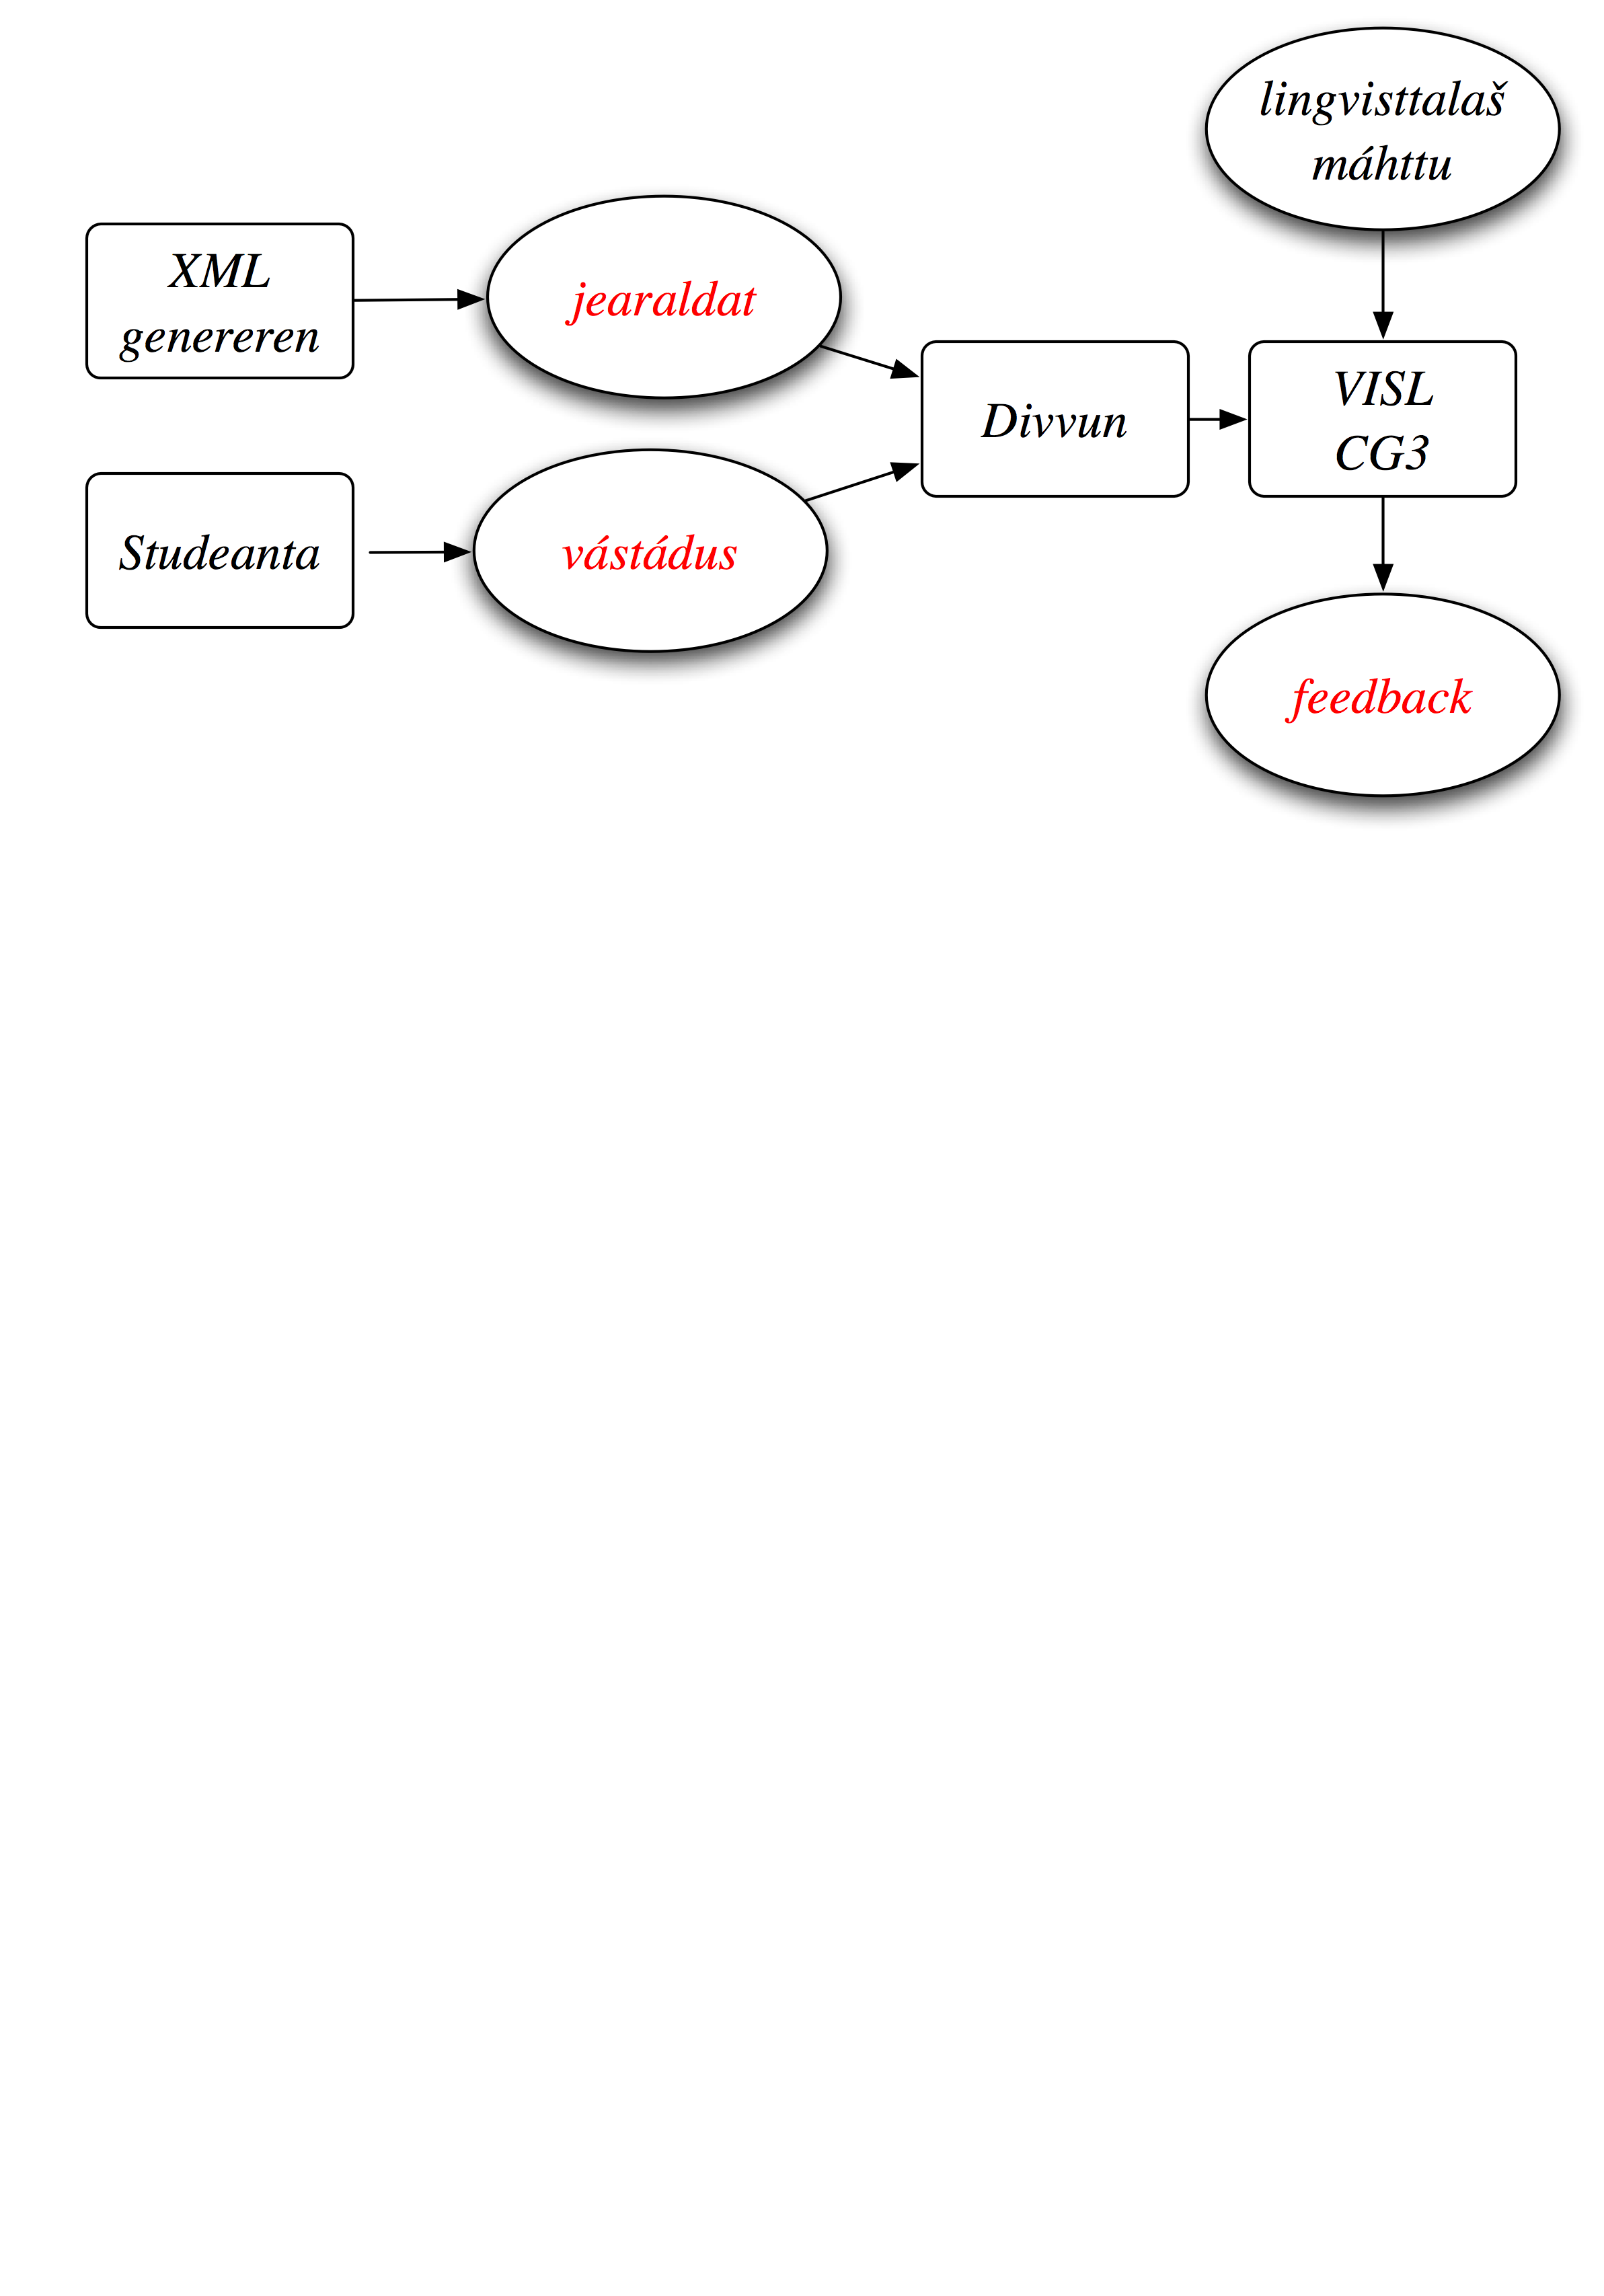
\includegraphics{img/skovi.png}} 
\newslide
We use our knowledge about:
\begin{itemize}
\item Sámi syntax
\item the learner´s interlanguage
\end{itemize}

\newslide
\textbf{Sámi syntax}\\
E.g. what can be in a NP:
\begin{itemize}
\item \small{NP: Gen (Num Attr) Gradeadv (A Attr) CC Gradeadv (A Attr) N}  		
\item what kind of agreement
\end{itemize}



\newslide
\textbf{Natural dialogue:} \\

\scalebox{0.40}[0.40]{
\includegraphics{img/lgiella1.png}} 

\newslide
\textbf{Natural dialogue:} \\

\scalebox{0.40}[0.40]{
\includegraphics{img/lgiella2.png}} 

\newslide
\textbf{Natural dialogue:} \\

\scalebox{0.40}[0.40]{
\includegraphics{img/lgiella3.png}} 
\newslide
\textbf{Natural dialogue:} \\

\scalebox{0.40}[0.40]{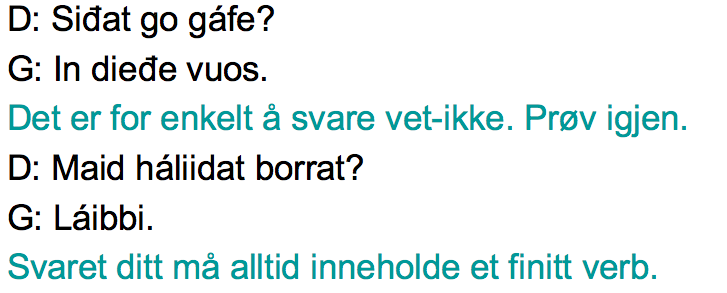
\includegraphics{img/lgiella4.png}} 
\newslide
\textbf{Natural dialogue:} \\

\scalebox{0.40}[0.40]{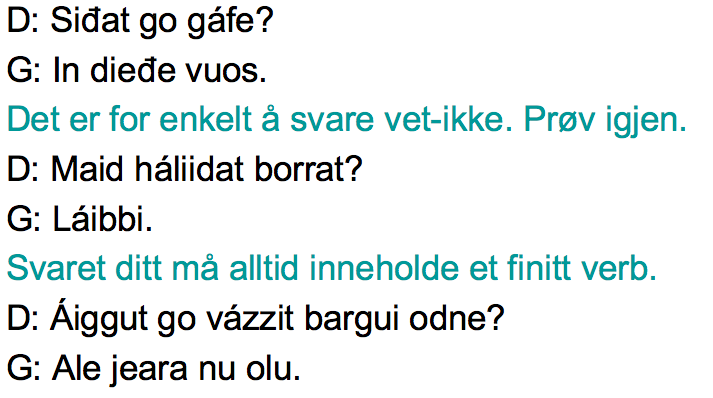
\includegraphics{img/lgiella5.png}} 
\newslide
\textbf{Natural dialogue:} \\

\scalebox{0.40}[0.40]{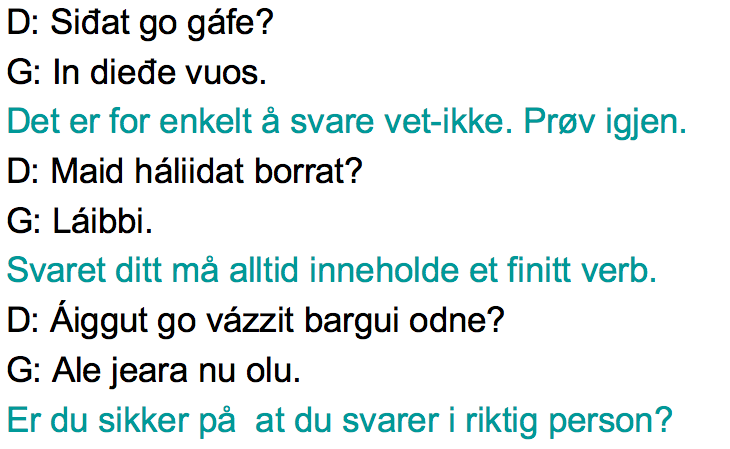
\includegraphics{img/lgiella6.png}} 


\newslide
\textbf{Problems -- 1: Didactics versus pragmatics} \\
The goal is to train morphology -- Solution:
\begin{itemize}
\item{No elipsis}
\item{The finite verb is compulsatory}
\item{Answer with the same verb when it is natural to do it}
\item{No inclusive 1st person dual and plural}
\item{The answer \textit{I do not know} is not accepted}
\end{itemize}




\newslide
\textbf{Problems -- 2} \\
only one finite verb in the clause: \\
\textit{*Mun áiggun vuolggán.}\\
\textit{Mun boran haman.}\\

In a finite-finite-construction:\\ -- the verbs should have same inflection\\
-- no adverb between\\
But this is not enough

\newslide
\textbf{Solution:} \\
Semantic set:\\
LIST INFV =  astat ádjánit áigut álgit beassat berret bivvat .... \\
\textnormal{*(INFV finite) + (VERB finite)}


\newslide
\textbf{Problems -- 3: Nominative versus accusative} \\
We cannot base our conclusion upon the word order, and the subject is not compulsory
\begin{itemize}
\item We can utilize the question - if it asks for an object (but it is still possible to answer without an object)
\end{itemize}
\newslide
\textbf{Solution:} \\
Semantic sets, e.g.: 
\begin{itemize}
\item verbs which have object as a compulsory argument (Strict Transitive Verbs)
\item verbs which cannot have a HUMAN as object
\end{itemize}

\newslide
\textbf{Can HUMAN be object?} \\

 \textit{borrat (eat)}   - HUMAN can be subject, not object \\
 
  \textit{lohkat (read)}  - the same, but a N Prop can be object, e.g.  \\ \textit{Mun lohken Fosse.}


\newslide
\textbf{Problems -- 4: Spelling error gives unintended lemma} \\
E.g.\textit{viessut}: \textit{viessut} Inf or \textit{viessat} Imprt \\
but we presuppose that the student want to write \textit{viesut} N Pl Nom. \\
Possible solutions:

\begin{itemize}
\item{Remove problematic lemmas and word forms}
\item{Ask the user: \\ Which one do you mean? \textit{viesut}  N or \textit{viessut} V }?
\end{itemize}


\newslide
\textbf{Problems -- 5: Spelling error gives unintended word form} \\
e.g. possessive suffixes vs. locative \\
\textit{biilas N Sg Nom Px Sg3 / biillas N Sg Loc} \\

Possible solutions:
\begin{itemize}
\item Remove possessive suffixes
\item Make comment to the user: \\
Mener du lokativ? I så fall er det feil stadieveksling.
\end{itemize}


%\newslide

%QA information retrieval how to process questions
%interactive, aske the user for clarification

%QA: 

%Question matrixes: generate a set of questions

%\newslide
%\textbf{Ovdamearka studeanttas}
%The output is manipulated  - it would not give two mappings to the same reading.
%\scalebox{.32}[.35]{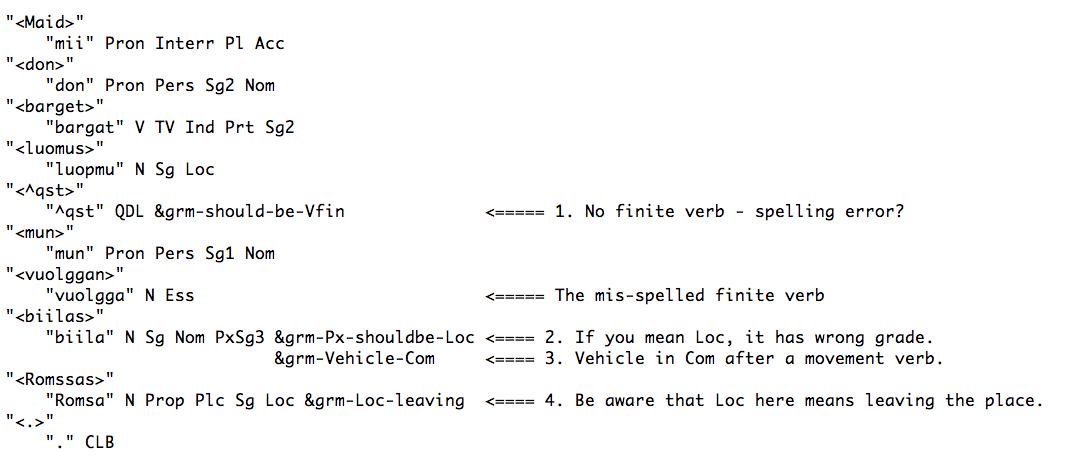
\includegraphics{img/sentence_example.png}}

\newslide
\textbf{Better that errors slip through than not accept what is correct} \\

- but what expectations does the user have?

\newslide
\textbf{Evaluation and improvement}\\
based on
\begin{itemize}
\item{Feedback from users}
\item{Feedback from teachers}
\item{Internet log}
\end{itemize}


\end{slide}
\end{document}




